\documentclass[conference]{IEEEtran}
\IEEEoverridecommandlockouts
\usepackage{cite}
\usepackage[bookmarks=false]{hyperref}
\usepackage{amsmath,amssymb,amsfonts}
\usepackage{graphicx}
\usepackage{float}
\usepackage{textcomp}
\usepackage{xcolor}
\usepackage{multirow}
\usepackage{array}
\usepackage{url}
\usepackage{booktabs}
\usepackage{tikz}
\usetikzlibrary{shapes.geometric, arrows, positioning, fit, arrows.meta}
\def\BibTeX{{\rm B\kern-.05em{\sc i\kern-.025em b}\kern-.08em
    T\kern-.1667em\lower.7ex\hbox{E}\kern-.125emX}}
\PassOptionsToPackage{bookmarks={false}}{hyperref}
\hypersetup{nolinks=true}
\hypersetup{final}
\setlength{\textfloatsep}{6pt plus 2pt minus 2pt}
\setlength{\intextsep}{6pt plus 2pt minus 2pt}
\setlength{\floatsep}{4pt plus 2pt minus 2pt}
\setlength{\abovecaptionskip}{3pt}
\setlength{\belowcaptionskip}{0pt}

\begin{document}

\title{A Comparative Evaluation of Topic Modeling Methods for Researcher-to-Research-Group Recommendation}

% \author{\IEEEauthorblockN{1\textsuperscript{st} Given Name Surname}
% \IEEEauthorblockA{\textit{dept. name of organization (of Aff.)} \\
% \textit{name of organization (of Aff.)}\\
% City, Country \\
% email address or ORCID}
% }

\maketitle

\begin{abstract}
Matching researchers with suitable research groups can support collaboration and researcher placement, but manual matching is difficult to apply at scale. Publication text provides evidence of research expertise, yet the relative value of classical and contextual topic models for this task remains unclear. This study presents a controlled comparison, rather than a new algorithm, of a BERTopic-based researcher-to-research-group recommendation framework against Latent Dirichlet Allocation (LDA) and Non-negative Matrix Factorization (NMF) under the same experimental pipeline, evaluated on 11,111 publication documents from 3,257 researchers across 12 computer science research groups. Topic vectors from titles and abstracts were averaged into researcher and group profiles and ranked by cosine similarity across 652 test researchers using top-$K$ metrics. BERTopic obtained the highest score on all 13 metrics, with an NDCG@5 of 0.736 and MRR of 0.809, though its margin over LDA was consistently narrow. NMF obtained the highest topic coherence (0.687) but ranked last on every recommendation metric, requiring only 18.8~s of total execution time against 180.3~s for LDA and 971.8~s for BERTopic. Topic coherence therefore does not reliably predict recommendation quality: BERTopic is preferable when ranking accuracy has priority and offline training is acceptable, LDA delivers quality close to BERTopic at a fraction of the cost, and NMF is fastest but least accurate, suiting resource-limited or frequently updated systems.
\end{abstract}
\vspace{0.25cm}

\begin{IEEEkeywords}
BERTopic, scholarly recommender systems, researcher profiling, scientific document analysis, ranking evaluation
\end{IEEEkeywords}

\section{Introduction}
\label{sec:intro}
Placing researchers in research groups that match their interests is difficult to perform manually and to scale, even though doing so well can support scientific collaboration, mentoring, and institutional planning~\cite{yang2014multilevel,sun2015raf}; as the number of researchers and groups grows, manual matching becomes increasingly subjective~\cite{zhang2023scholarly}. Scholarly recommender systems have addressed related tasks through content-based and interaction-based methods~\cite{zhang2023scholarly,bai2019scientific}, but interaction data such as co-authorship and citation links may be sparse for new researchers. Publication titles and abstracts instead provide direct evidence of current research interests and can support recommendations without prior interaction records~\cite{bai2019scientific,beel2016research}.

Topic modeling converts publication text into compact thematic representations using three common paradigms: probabilistic models such as LDA~\cite{jelodar2019lda,blei2003lda}, matrix-factorization models such as NMF~\cite{lee2000nmf}, and contextual embedding-based models such as BERTopic, which combines document embeddings, dimensionality reduction, density-based clustering, and class-based TF-IDF~\cite{grootendorst2022bertopic}. Previous studies have compared these families on social media, online communities, news, and other short-text collections~\cite{egger2022topic,kaur2024moving,babalola2024comprehensive}, but most have assessed topic interpretability or clustering behavior rather than the value of topic vectors inside a downstream recommendation task.

This creates two related gaps: existing studies have not established how LDA, NMF, and BERTopic compare under identical profile construction, similarity ranking, and researcher-level evaluation for researcher-to-research-group recommendation, and model selection has often relied on intrinsic topic coherence rather than this kind of controlled comparison, although prior work has questioned whether higher coherence predicts better downstream performance~\cite{roder2015exploring,rudiger2022topic}. These gaps motivate two research questions: (1) how do LDA, NMF, and BERTopic compare when used to rank research groups for a test researcher under one identical pipeline, and (2) does a topic model's intrinsic coherence agree with its downstream recommendation quality?

This study addresses these questions through a comparative evaluation of LDA, NMF, and BERTopic for publication-based researcher-to-research-group recommendation, evaluating 11,111 prepared publication documents from 3,257 researchers across 12 research groups using a researcher-level train-test split with group profiles built only from training researchers. As reported in Section~\ref{sec:results}, the answers diverge: the model with the most coherent topics is not the model with the best research-group rankings, indicating that coherence alone is not a reliable criterion for selecting a topic representation for this task. The main contributions are:
\begin{enumerate}
    \item A comparative evaluation of probabilistic, matrix-factorization, and contextual topic representations under the same profile construction, cosine-similarity ranking, and test protocol.
    \item A standardized researcher-level evaluation procedure in which test researchers remain separate from model fitting and group-profile construction.
    \item An analysis of the relationship between $C_v$ topic coherence and 13 recommendation metrics, including Precision, Recall, F1-score, NDCG, and MRR.
    \item A paired per-researcher significance analysis (Wilcoxon signed-rank tests) quantifying which observed ranking differences between models are statistically robust rather than attributable to sampling variation in the single split.
\end{enumerate}


\section{Related Works}
\label{sec:related}
\subsection{Scholarly and Researcher Recommendation}
Scholarly recommendation has covered papers, experts, collaborators, reviewers, venues, and research groups, combining researcher profiles with multilevel information mining~\cite{yang2014multilevel,sun2015raf} and grouping methods into content-based, collaborative, graph-based, and hybrid approaches~\cite{zhang2023scholarly,bai2019scientific,beel2016research,marcuzzo2022recommendation}. Interaction-based methods represent collaboration patterns but are less useful when historical links are unavailable; publication-based profiling avoids this, as in the Semantic Academic Profiler~\cite{viegas2022semantic}. These studies support publication-based representation, but almost none directly compare several topic models for ranking research groups under one pipeline -- a gap the comparative literature reviewed next has not filled, having instead concentrated on domains outside scholarly recommendation.

\subsection{Topic Modeling for Scholarly Text}
Topic modeling provides one family of content representations for scholarly text: LDA remains a common probabilistic model for latent themes~\cite{jelodar2019lda,blei2003lda}, NMF represents documents through non-negative matrix decomposition~\cite{lee2000nmf}, and BERTopic combines contextual embeddings beyond word co-occurrence~\cite{vaswani2017attention} with UMAP, HDBSCAN, and class-based TF-IDF~\cite{grootendorst2022bertopic}. Domain-adapted embeddings such as SciBERT~\cite{beltagy2019scibert} and the citation-informed SPECTER embeddings used here~\cite{cohan2020specter} better capture scientific-publication semantics than general-domain embeddings, motivating BERTopic's SPECTER-based encoder.

Comparative studies have evaluated LDA, NMF, BERTopic, and related models on short, non-scholarly text such as Twitter posts, online communities, and news headlines, using topic diversity, coherence, or classification accuracy~\cite{egger2022topic,kaur2024moving,babalola2024comprehensive,laureate2023systematic}. Closer to the present domain, Rumadi et al.~\cite{rumadi2025coherence} compared topic coherence across LDA, NMF, BERTopic, and Top2Vec on scientific literature, extending this literature to scholarly text; even this closest prior work, however, evaluates only intrinsic coherence and not a downstream ranking task. Together, this literature shows that model behavior depends on the corpus and evaluation objective without establishing which representation is most useful once publication vectors are aggregated into researcher and research-group profiles. Content-based recommender systems have long compared mean-pooled item or user vectors by cosine similarity to rank candidates~\cite{lops2011content} -- the same mechanism adopted here -- but it has not previously been evaluated with topic vectors from probabilistic, matrix-factorization, and contextual models side by side.

\subsection{Topic Coherence and Downstream Evaluation}
Topic coherence has often been used to select and compare topic models; measures such as $C_v$ estimate whether leading topic words occur in a semantically consistent context~\cite{roder2015exploring,mimno2011optimizing}, though strong intrinsic quality does not necessarily predict downstream performance~\cite{rudiger2022topic}. Recommendation evaluation instead measures whether relevant items appear near the top of a ranked list, using Precision, Recall, F1-score, NDCG, and MRR~\cite{valcarce2020assessing}. These have largely been studied as separate concerns; Section~\ref{sec:results} revisits the separation by reporting both $C_v$ coherence and 13 recommendation metrics for the same three models.


\section{Methodology}
\label{sec:methodology}
This study developed a BERTopic-based framework for researcher-to-research-group recommendation and compared it with LDA and NMF under one experimental pipeline (Fig.~\ref{fig:framework}): publication-level topic vectors were averaged into researcher profiles, training-researcher profiles formed the group profiles, and cosine similarity between these profiles produced the ranked recommendations.

\begin{figure}[t]
\centering
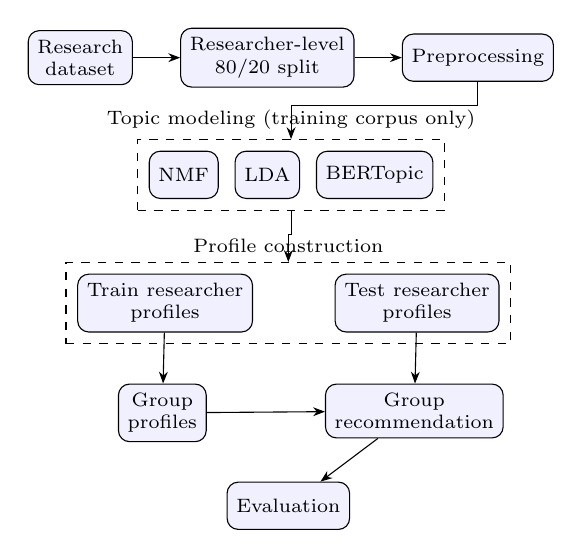
\begin{tikzpicture}[
    node distance=6mm and 6mm,
    box/.style={draw, rounded corners, align=center, minimum height=6mm, font=\scriptsize, fill=blue!6},
    grp/.style={draw, dashed, inner sep=4pt},
    arr/.style={-{Stealth[length=1.5mm]}}
]
\node[box] (data) {Research\\dataset};
\node[box, right=of data] (split) {Researcher-level\\80/20 split};
\node[box, right=of split] (prep) {Preprocessing};

\node[box, below=8mm of split] (lda) {LDA};
\node[box, left=2mm of lda] (nmf) {NMF};
\node[box, right=2mm of lda] (bert) {BERTopic};
\node[grp, fit=(nmf)(lda)(bert), label={[font=\scriptsize]above:Topic modeling (training corpus only)}] (tm) {};

\node[box, below=8mm of tm.south, xshift=-16mm] (trp) {Train researcher\\profiles};
\node[box, below=8mm of tm.south, xshift=16mm] (tep) {Test researcher\\profiles};
\node[grp, fit=(trp)(tep), label={[font=\scriptsize]above:Profile construction}] (pc) {};

\node[box, below=5mm of pc.south, xshift=-16mm] (gp) {Group\\profiles};
\node[box, below=5mm of pc.south, xshift=16mm] (rec) {Group\\recommendation};
\node[box, below=5mm of gp.south, xshift=16mm] (ev) {Evaluation};

\draw[arr] (data) -- (split);
\draw[arr] (split) -- (prep);
\draw[arr] (prep.south) -- ++(0,-3mm) -| (tm.north);
\draw[arr] (trp) -- (gp);
\draw[arr] (tep) -- (rec);
\draw[arr] (gp) -- (rec);
\draw[arr] (rec) -- (ev);
\draw[arr] (tm.south) -- ++(0,-3mm) -| (pc.north);
\end{tikzpicture}
\caption{Research framework. Data collection, the researcher-level split, and preprocessing are shared across models; LDA, NMF, and BERTopic are then fit only on the training corpus, so the topic representation is the only model-dependent stage in an otherwise identical profile-construction, cosine-similarity ranking, and evaluation pipeline.}
\label{fig:framework}
\end{figure}

\subsection{Data Source}
Researchers and research group data were obtained from CSRankings, publication metadata from DBLP, and abstracts from Semantic Scholar; each record contained a title, abstract, author list, publication year, venue, and DOI when available. The CSRankings research areas defined 12 target research groups. After data validation and preprocessing, the dataset contained 11,111 publication documents from 3,257 researchers, divided into 2,605 training and 652 test researchers using an 80/20 researcher-level split (seed 42) that kept every publication by one researcher in the same partition.

\subsection{Data Preprocessing}
Each publication document combined its title and abstract; records without usable text or a labeled researcher were excluded. LDA and NMF used bag-of-words text converted to lowercase and stripped of punctuation, non-alphanumeric tokens, common English stopwords, and a small set of generic publication terms (e.g., ``abstract,'' ``paper,'' ``conference,'' ``journal,'' ``manuscript'') that carry no topical information. BERTopic used the original title-and-abstract text with normalized whitespace to preserve information required by the embedding model. Vectorizers were fitted only on training publications, with vocabulary limited to 20,000 features and minimum/maximum document frequencies of 2 and 0.8.

\subsection{Hyperparameter Optimization}
Hyperparameters were selected using only the training corpus, ranking candidate configurations by topic coherence; the reported grids reflect the final stage of a staged coarse-to-fine search, with the highest-scoring configuration for each model used in the final experiment. The search varied the number of topics for LDA and NMF and, for BERTopic, the HDBSCAN minimum topic size and number of UMAP neighbors. The selected settings were 29 topics and 20 iterations for LDA, 11 topics and 800 iterations for NMF, and for BERTopic a minimum topic size of 45, 50 UMAP neighbors, five UMAP components, and a minimum distance of 0.0. Final recommendation metrics were calculated on the held-out researchers. All models used random seed 42 where supported: LDA, NMF, and UMAP's \texttt{random\_state} were seeded directly; HDBSCAN does not expose a random seed and is deterministic for fixed embeddings and parameters.

\subsection{Topic Modeling}
LDA, NMF, and BERTopic were fitted to the same training partition, each producing a topic vector for every training and test publication. LDA (scikit-learn's \texttt{LatentDirichletAllocation}) fitted a probabilistic model to document-term count vectors with batch learning, representing each publication as a probability distribution over 29 latent topics. NMF (scikit-learn's \texttt{NMF}) decomposed a TF-IDF document-term matrix into non-negative document-topic and topic-term matrices using NNDSVDa initialization, yielding an 11-dimensional document-topic vector per publication; fitted training vectorizers transformed test publications without refitting. BERTopic encoded publication text with the pretrained \texttt{allenai/specter} model (\texttt{sentence-transformers}); UMAP (\texttt{umap-learn}) reduced the embeddings using cosine distance, and HDBSCAN (\texttt{hdbscan}) formed topic clusters, orchestrated through the \texttt{BERTopic} package. Outliers were reassigned through embedding similarity and topics updated with the same vectorizer for consistency. BERTopic's \texttt{approximate\_distribution()} generated a document-topic probability distribution per publication, used in the recommendation stage rather than single topic labels.

\subsection{Profile Construction}
All profiles were constructed in the topic space produced by the corresponding model. Let $D_r = \{d_1, d_2, \dots, d_n\}$ denote the publications of researcher $r$, and let $v_d$ be the topic vector of publication $d$. The researcher profile was the arithmetic mean of the publication vectors:
\begin{equation}
R_r = \frac{1}{|D_r|} \sum_{d \in D_r} v_d
\label{eq:profile}
\end{equation}
This operation produced one topic profile for each researcher. Research group profiles were built only from training researchers. For a research group with training members $G = \{r_1, r_2, \dots, r_m\}$, the group profile was
\begin{equation}
P_G = \frac{1}{|G|} \sum_{r \in G} R_r
\label{eq:group}
\end{equation}
where $R_r$ was the profile of member $r$. Restricting this aggregation to training members prevented test researcher profiles from entering the group representations.

\subsection{Research Group Recommendation}
Each test researcher profile was compared with all 12 research group profiles using cosine similarity,
\begin{equation}
\mathrm{sim}(R_r, P_G) = \frac{R_r \cdot P_G}{\lVert R_r \rVert \, \lVert P_G \rVert}
\label{eq:cosine}
\end{equation}
where $R_r$ is the profile of test researcher $r$ from \eqref{eq:profile} and $P_G$ is the profile of research group $G$ from \eqref{eq:group}. The groups were sorted by decreasing similarity, with an alphabetical secondary order for equal scores. The same ranking procedure was applied to LDA, NMF, and BERTopic profiles, so the topic representation was the only model-dependent part of the recommendation pipeline. The system returned a ranked list rather than a single group because a researcher could have more than one ground-truth research group.

\subsection{Evaluation}
The ranked groups for each of the 652 test researchers were compared with that researcher's known CSRankings group memberships using Precision@$K$, Recall@$K$, F1-score@$K$, and NDCG@$K$ at $K=1,3,5$: Precision is the proportion of the first $K$ recommendations that were relevant, Recall the proportion of relevant groups retrieved within the first $K$, F1-score their harmonic mean, and NDCG assigns greater value to relevant groups near the top of the ranking; mean reciprocal rank (MRR) measures the inverse rank of the first relevant group. Each metric was the arithmetic mean of per-researcher scores, using the same split, group candidates, profile construction, ranking method, and metrics for all three models.

\subsection{Statistical Significance Testing}
\label{sec:sigtest}
Because all metrics were computed on one fixed 80/20 split, cutoff-based Precision, Recall, F1-score, NDCG, and MRR were additionally compared between each model pair using a two-sided Wilcoxon signed-rank test over the 652 matched per-researcher scores; this paired design controls for researcher-level variation since the same test researchers and ground-truth labels were scored by every model. Tied scores contributed a zero difference and were excluded, following the conventional zero-difference handling. Because 13 metrics were tested per model pair, a Bonferroni-corrected threshold of $\alpha = 0.05/13 \approx 0.0038$ is reported alongside the uncorrected $\alpha = 0.05$ to guard against inflated false positives.


\section{Results and Discussion}
\label{sec:results}
\subsection{Dataset}
The prepared dataset contained 11,111 unique publication documents from 3,257 researchers, split into 2,605 training and 652 test researchers. Fig.~\ref{fig:dataset}(a) showed large differences in group membership: Machine Learning was largest (2,480 researchers), followed by Artificial Intelligence (2,090) and Computer Vision (1,748), while Visualization (118) and Software Engineering (127) were smallest; counts exceed the number of unique researchers because one researcher could belong to several groups. Publication profile size was also uneven (Fig.~\ref{fig:dataset}(b)): a mean of 6.1 publications per researcher and a median of 2, ranging from 1 to 59, with the gap between mean and median and the long right tail showing that most researchers had short profiles while a smaller number had many.

Fig.~\ref{fig:dataset}(c) described the multi-label structure of the task: only 421 researchers (13\%) belonged to one group, membership in three groups was most common (703 researchers, 22\%), two and four groups accounted for about 18\% and 20\%, and the remainder belonged to five or more groups, including nine researchers with nine labels -- representing researcher placement as a ranked multi-group problem rather than single-label classification.

\begin{figure}[t]
    \centering
    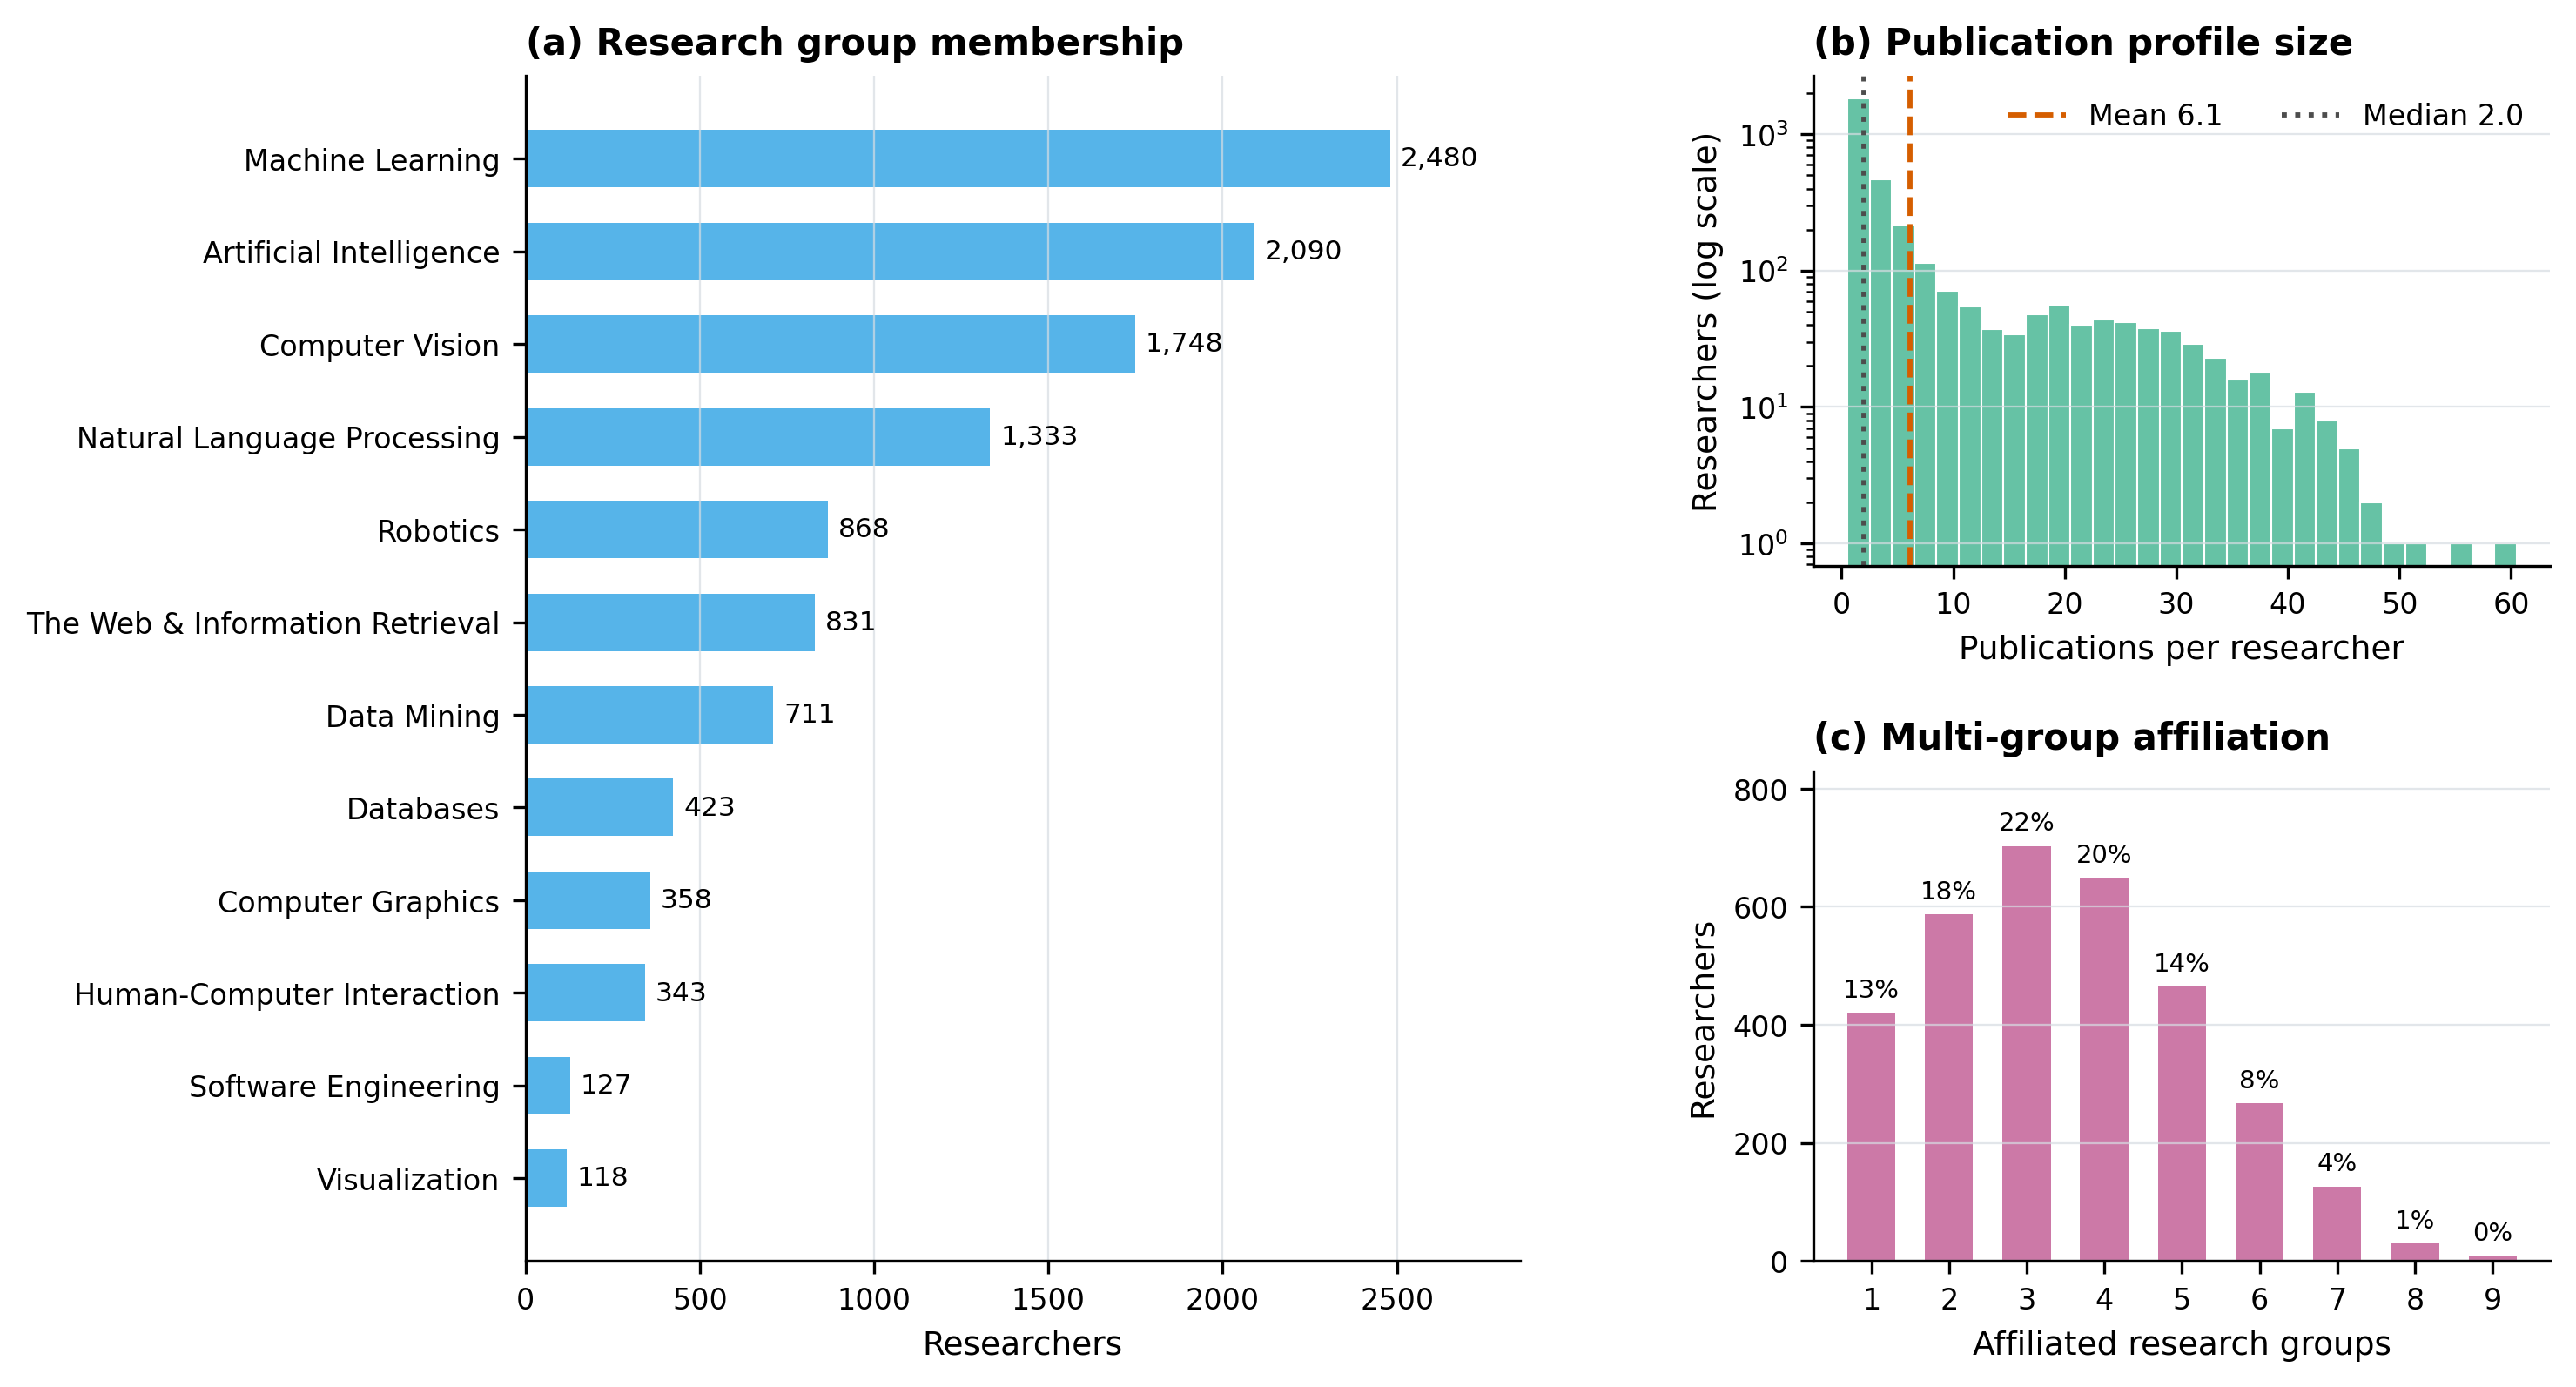
\includegraphics[width=0.94\columnwidth]{sections/figures/02_dataset_characterization.png}
    \caption{Dataset characteristics: (a) researcher membership in each group, (b) the distribution of publication profile sizes, and (c) the number of research group affiliations per researcher.}
    \label{fig:dataset}
\end{figure}

\subsection{Hyperparameter Optimization}
Fig.~\ref{fig:hpsearch} reported the training-corpus $C_v$ coherence obtained during the parameter search. For LDA, the highest coherence (0.521625) was obtained with 29 topics, against 0.512700--0.518153 for the other three tested counts. For NMF, the best configuration (11 topics) reached 0.686782, against 0.683174 for 9 topics and lower values for 12 and 15. The BERTopic search covered nine combinations of minimum topic size and UMAP neighbors: a minimum topic size of 45 with 50 neighbors ranked first (0.659480, 43 topics), close to 45/55 neighbors (0.658543), while two configurations at 60 neighbors produced only five topics and the lowest coherence (0.533384); all configurations reported zero remaining noise documents after outlier reassignment. The rank-one configuration for each model was used in the final experiment.

\begin{figure}[t]
    \centering
    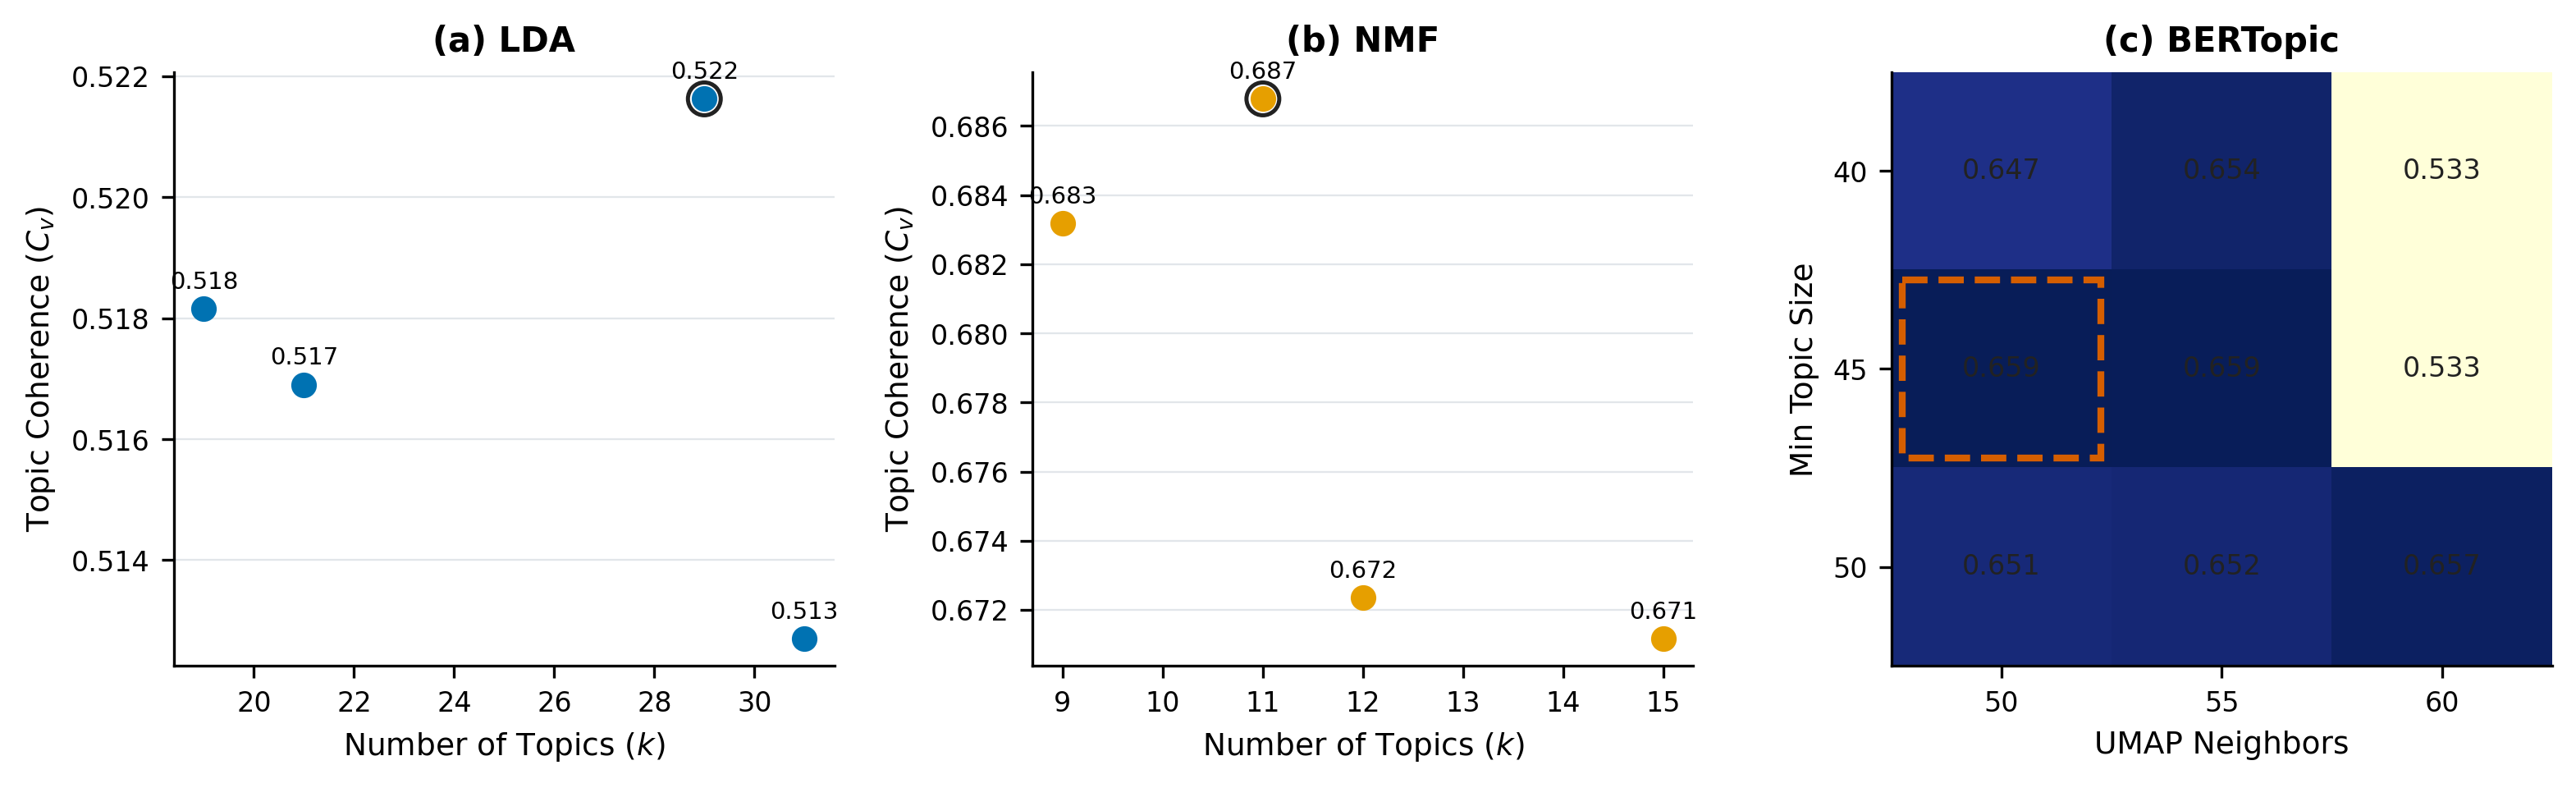
\includegraphics[width=0.94\columnwidth]{sections/figures/03_hyperparameter_search.png}
    \caption{Training-corpus hyperparameter search.}
    \label{fig:hpsearch}
\end{figure}

\subsection{Recommendation Performance}
Table~\ref{tab:main} summarizes the main test results at $K=5$ and MRR, together with paired Wilcoxon signed-rank tests (Section~\ref{sec:sigtest}) against BERTopic. BERTopic obtained the highest value in every metric, reaching an NDCG@5 of 0.736 and MRR of 0.809 against 0.719/0.793 for LDA and 0.640/0.774 for NMF. Fig.~\ref{fig:recperf} extends the comparison to Precision, Recall, F1-score, and NDCG at $K=1,3,5$: BERTopic ranked first in all 12 cutoff-based metrics; Precision decreased and Recall increased as more groups were returned, F1-score rose because the gain in Recall exceeded the loss in Precision, and NDCG stayed above 0.60 for every model and cutoff. Across all 13 reported metrics, BERTopic ranked first, LDA second, and NMF third.

\begin{table}[t]
\caption{Recommendation Performance ($K{=}5$, MRR) and Paired Wilcoxon Tests vs.\ BERTopic (BT), $n=652$}
\label{tab:main}
\centering
\scriptsize
\setlength{\tabcolsep}{3pt}
\begin{tabular}{lrrrrrrr}
\toprule
 & & & & \multicolumn{2}{c}{BT$-$LDA} & \multicolumn{2}{c}{BT$-$NMF} \\
Metric & LDA & NMF & BT & $\Delta$ & $p$-value & $\Delta$ & $p$-value \\
\midrule
P@5    & 0.4966 & 0.4301 & 0.5080 & 0.0113 & 0.097 & 0.0779 & $<0.001^{*}$ \\
R@5    & 0.7647 & 0.6770 & 0.7824 & 0.0177 & 0.007$^{*}$ & 0.1054 & $<0.001^{*}$ \\
F1@5   & 0.5652 & 0.4923 & 0.5790 & 0.0138 & 0.007$^{*}$ & 0.0867 & $<0.001^{*}$ \\
NDCG@5 & 0.7199 & 0.6405 & 0.7362 & 0.0163 & 0.073 & 0.0957 & $<0.001^{*}$ \\
MRR    & 0.7932 & 0.7750 & 0.8093 & 0.0160 & 0.113 & 0.0343 & 0.003$^{*}$ \\
\bottomrule
\end{tabular}
\vspace{2pt}

\raggedright\scriptsize $^{*}$Significant at uncorrected $\alpha=0.05$. None of the BT-vs-LDA comparisons survive the Bonferroni threshold $\alpha\approx0.0038$ (13 tests); all BT-vs-NMF comparisons do.
\end{table}

\begin{figure}[t]
    \centering
    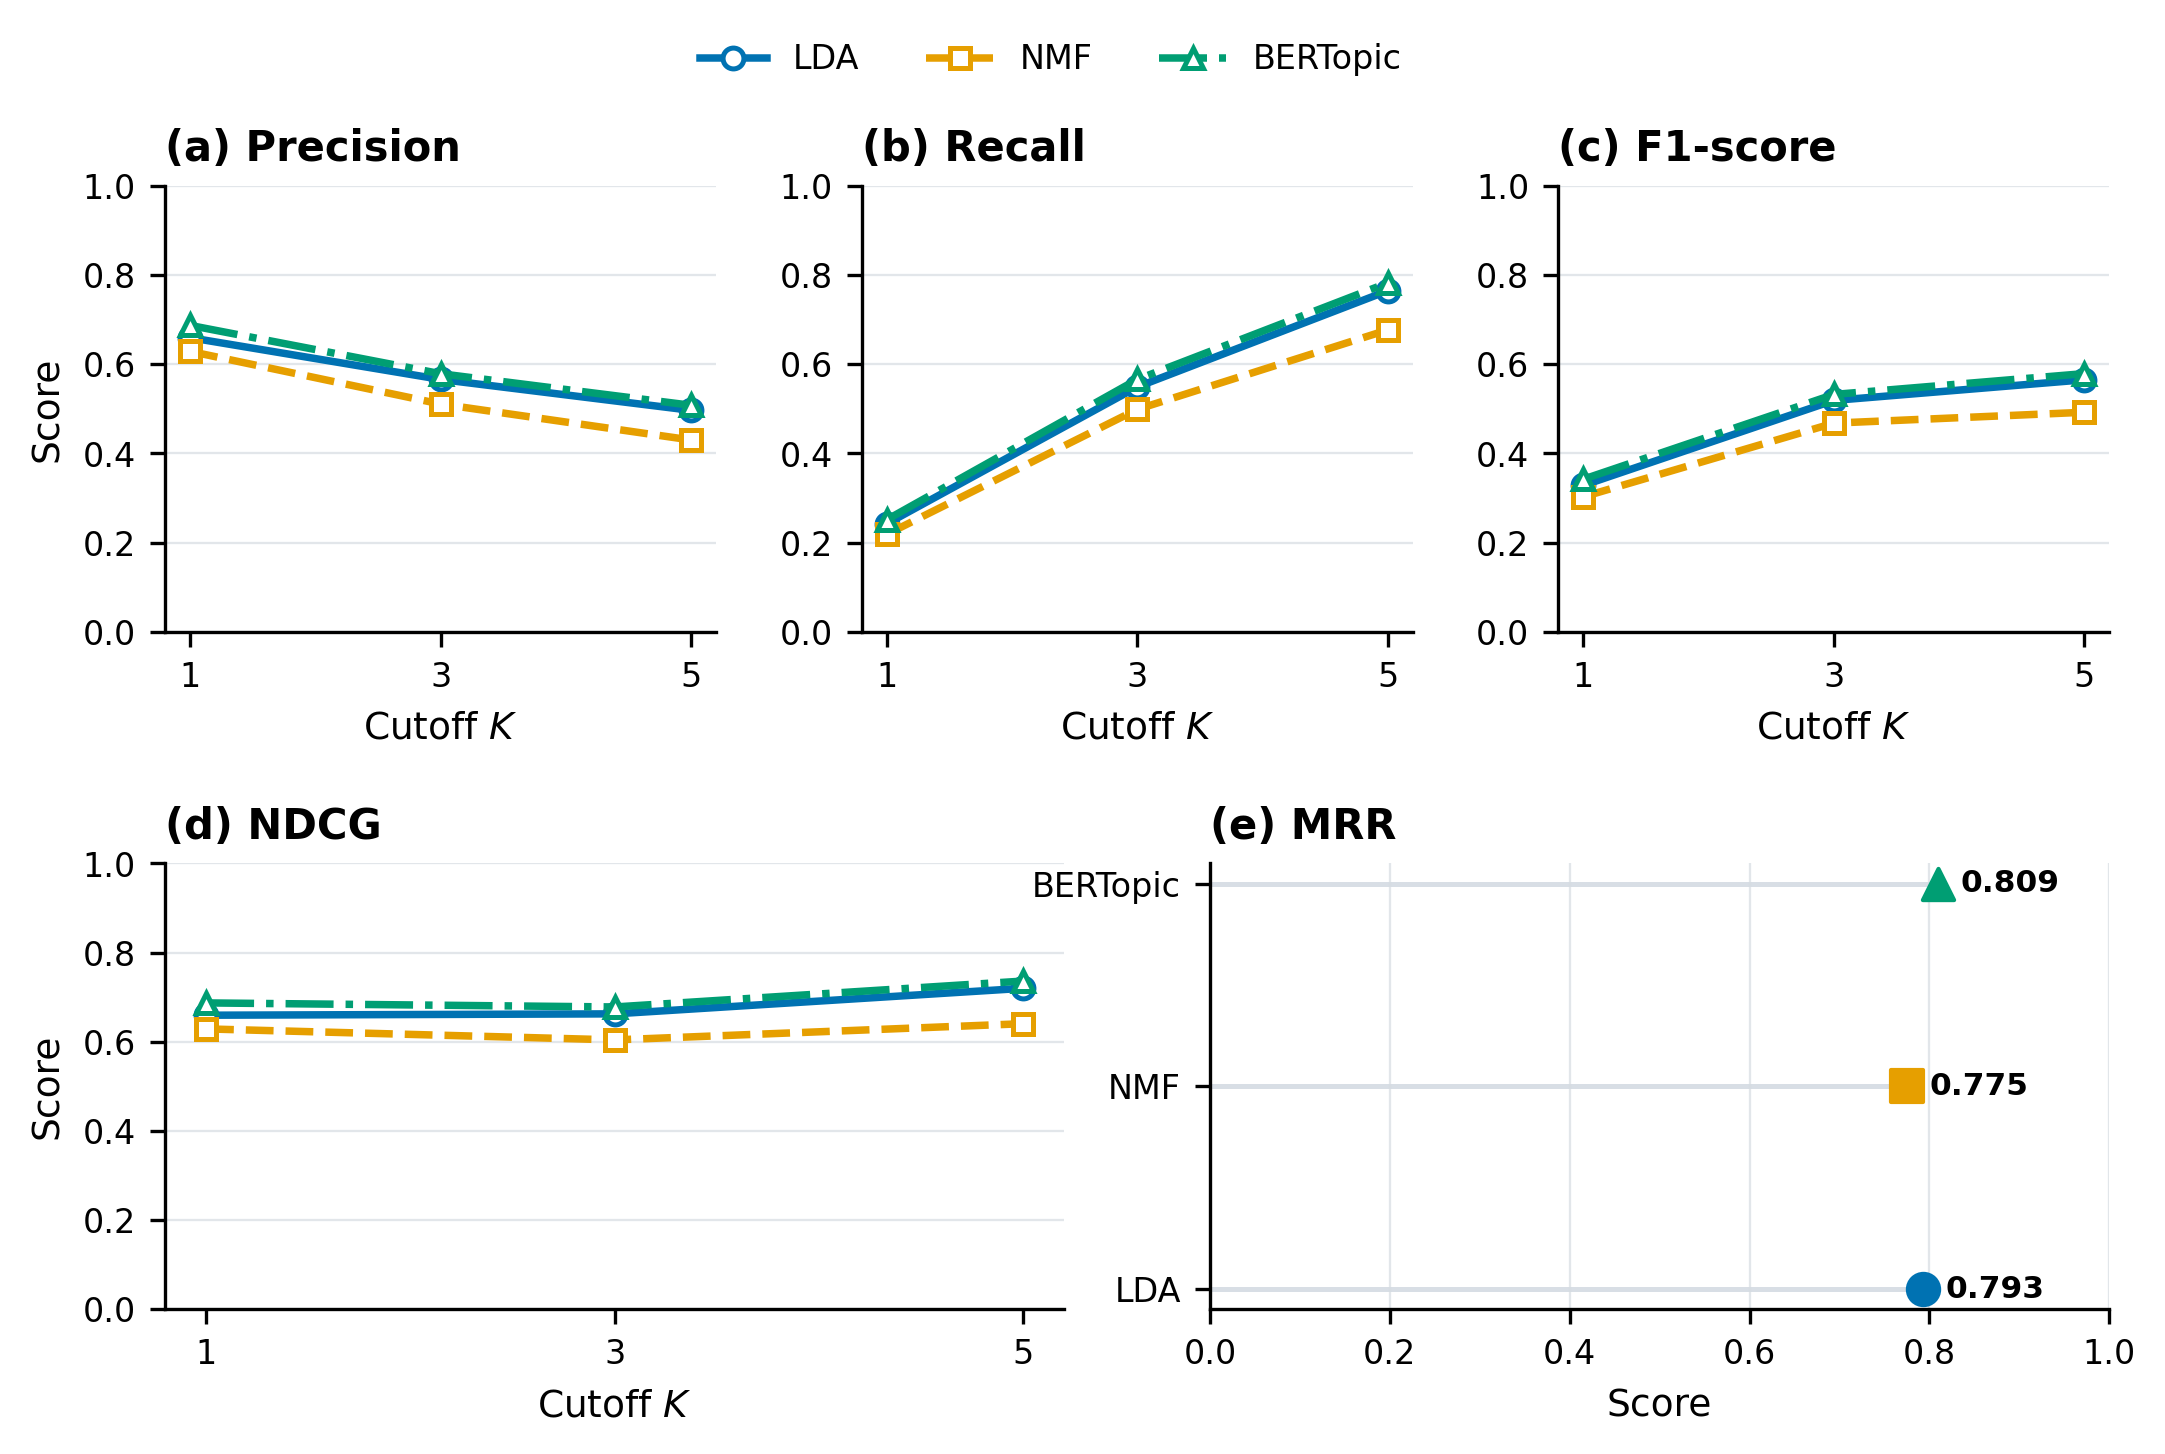
\includegraphics[width=0.94\columnwidth]{sections/figures/04_recommendation_performance.png}
    \caption{Recommendation performance.}
    \label{fig:recperf}
\end{figure}

BERTopic's advantage over NMF was statistically significant for every tested metric, surviving the Bonferroni-corrected threshold; its advantage over LDA was smaller, reaching nominal significance ($p<0.05$) only for Recall@5 and F1@5, with none of the five comparisons surviving Bonferroni correction. Across the complete set of 13 metrics, BERTopic differed significantly from LDA on 3 of 13 (23\%) and from NMF on 13 of 13 (100\%) at the uncorrected threshold: it ranks numerically first on every metric, but only its separation from NMF is statistically robust on this split, while its separation from LDA is a consistent yet comparatively fragile signal.

BERTopic's advantage may relate to its SPECTER embeddings, which represent scientific publications in a contextual semantic space that keeps related publications close even across different terms. Unlike LDA and NMF, fitted only on the roughly 11,000-document training corpus, SPECTER was pretrained on a much larger external corpus of scientific publications, so part of BERTopic's advantage may reflect this external pretraining signal rather than the topic-modeling mechanism itself; the experiment did not isolate the embedding, dimensionality-reduction, clustering, and outlier-reassignment components, so the difference cannot be assigned to one component alone.

\subsection{Topic Quality and Computational Runtime}
Fig.~\ref{fig:quality}(a) compared the final topic coherence values: NMF was highest (0.686782), followed by BERTopic (0.659480) and LDA (0.521625) -- an order that differs from the recommendation results, where NMF ranked last and BERTopic best despite the second-highest coherence. This mismatch suggests that $C_v$, which evaluates co-occurrence of leading words, and recommendation quality, which depends on whether complete topic vectors separate researcher and group profiles after aggregation, measure different properties; a model can produce coherent topic words without the most useful ranking representation, consistent with prior evidence that intrinsic topic metrics do not always predict downstream performance~\cite{rudiger2022topic}.

Runtime (Fig.~\ref{fig:quality}(b)) also differed substantially: NMF was fastest (18.1~s training, 0.7~s inference), LDA required 178.5~s/1.8~s, and BERTopic 966.5~s/5.2~s, for total execution times of 18.8~s, 180.3~s, and 971.8~s respectively (unrounded per-stage totals can differ by up to 0.1~s from the one-decimal figures above, e.g.\ BERTopic's 971.777~s rounds to 971.8~s though 966.5~s+5.2~s sums to 971.7~s). Training accounted for most of the measured time for every model.

\begin{figure}[t]
    \centering
    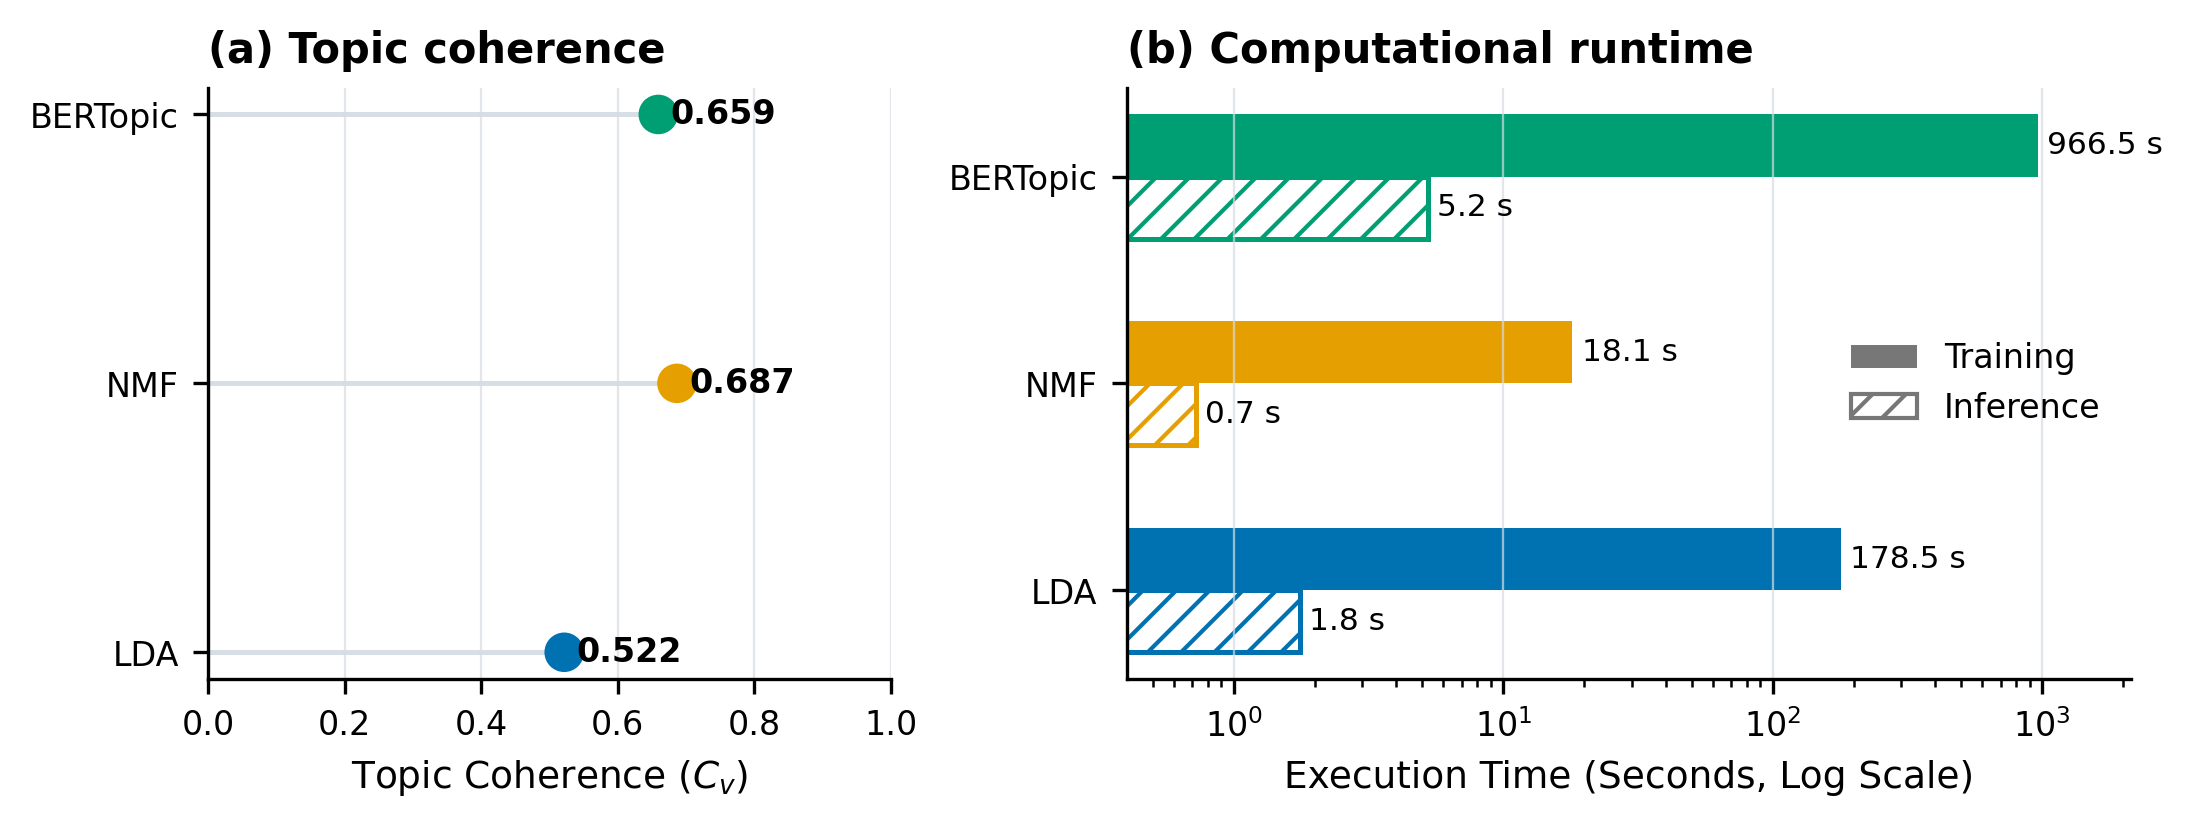
\includegraphics[width=0.94\columnwidth]{sections/figures/05_model_quality_and_runtime.png}
    \caption{Model characteristics: (a) topic coherence and (b) computational runtime.}
    \label{fig:quality}
\end{figure}

This pattern shows a clear quality/cost trade-off: BERTopic is preferable when ranking accuracy has priority and training can run offline, NMF when frequent retraining or limited resources matter, and LDA occupies a middle position with quality close to BERTopic at lower cost. Hardware and dependency-version details for this run were not recorded, so these figures should be read as indicative of relative model cost rather than an absolute, reproducible benchmark.

\subsection{Performance Across Research Groups}
Fig.~\ref{fig:pergroup} reported Top-3 precision per research group; performance varied more across groups than across models within a group. Machine Learning and Computer Vision had the highest values (approximately 0.91 and 0.86--0.89), followed by Artificial Intelligence and Natural Language Processing (0.63--0.74). The middle and lower rows showed wider separation: BERTopic led The Web and Information Retrieval (0.59), Databases (0.54), and Human-Computer Interaction (0.44); NMF led Robotics (0.60) and Data Mining (0.44); LDA led Natural Language Processing (0.74). No model ranked first for every group: counting the highest or tied-highest score across the 12 groups, BERTopic led in 6 (including a tie with LDA in Machine Learning), LDA in 4, and NMF in 3.

\begin{figure}[t]
    \centering
    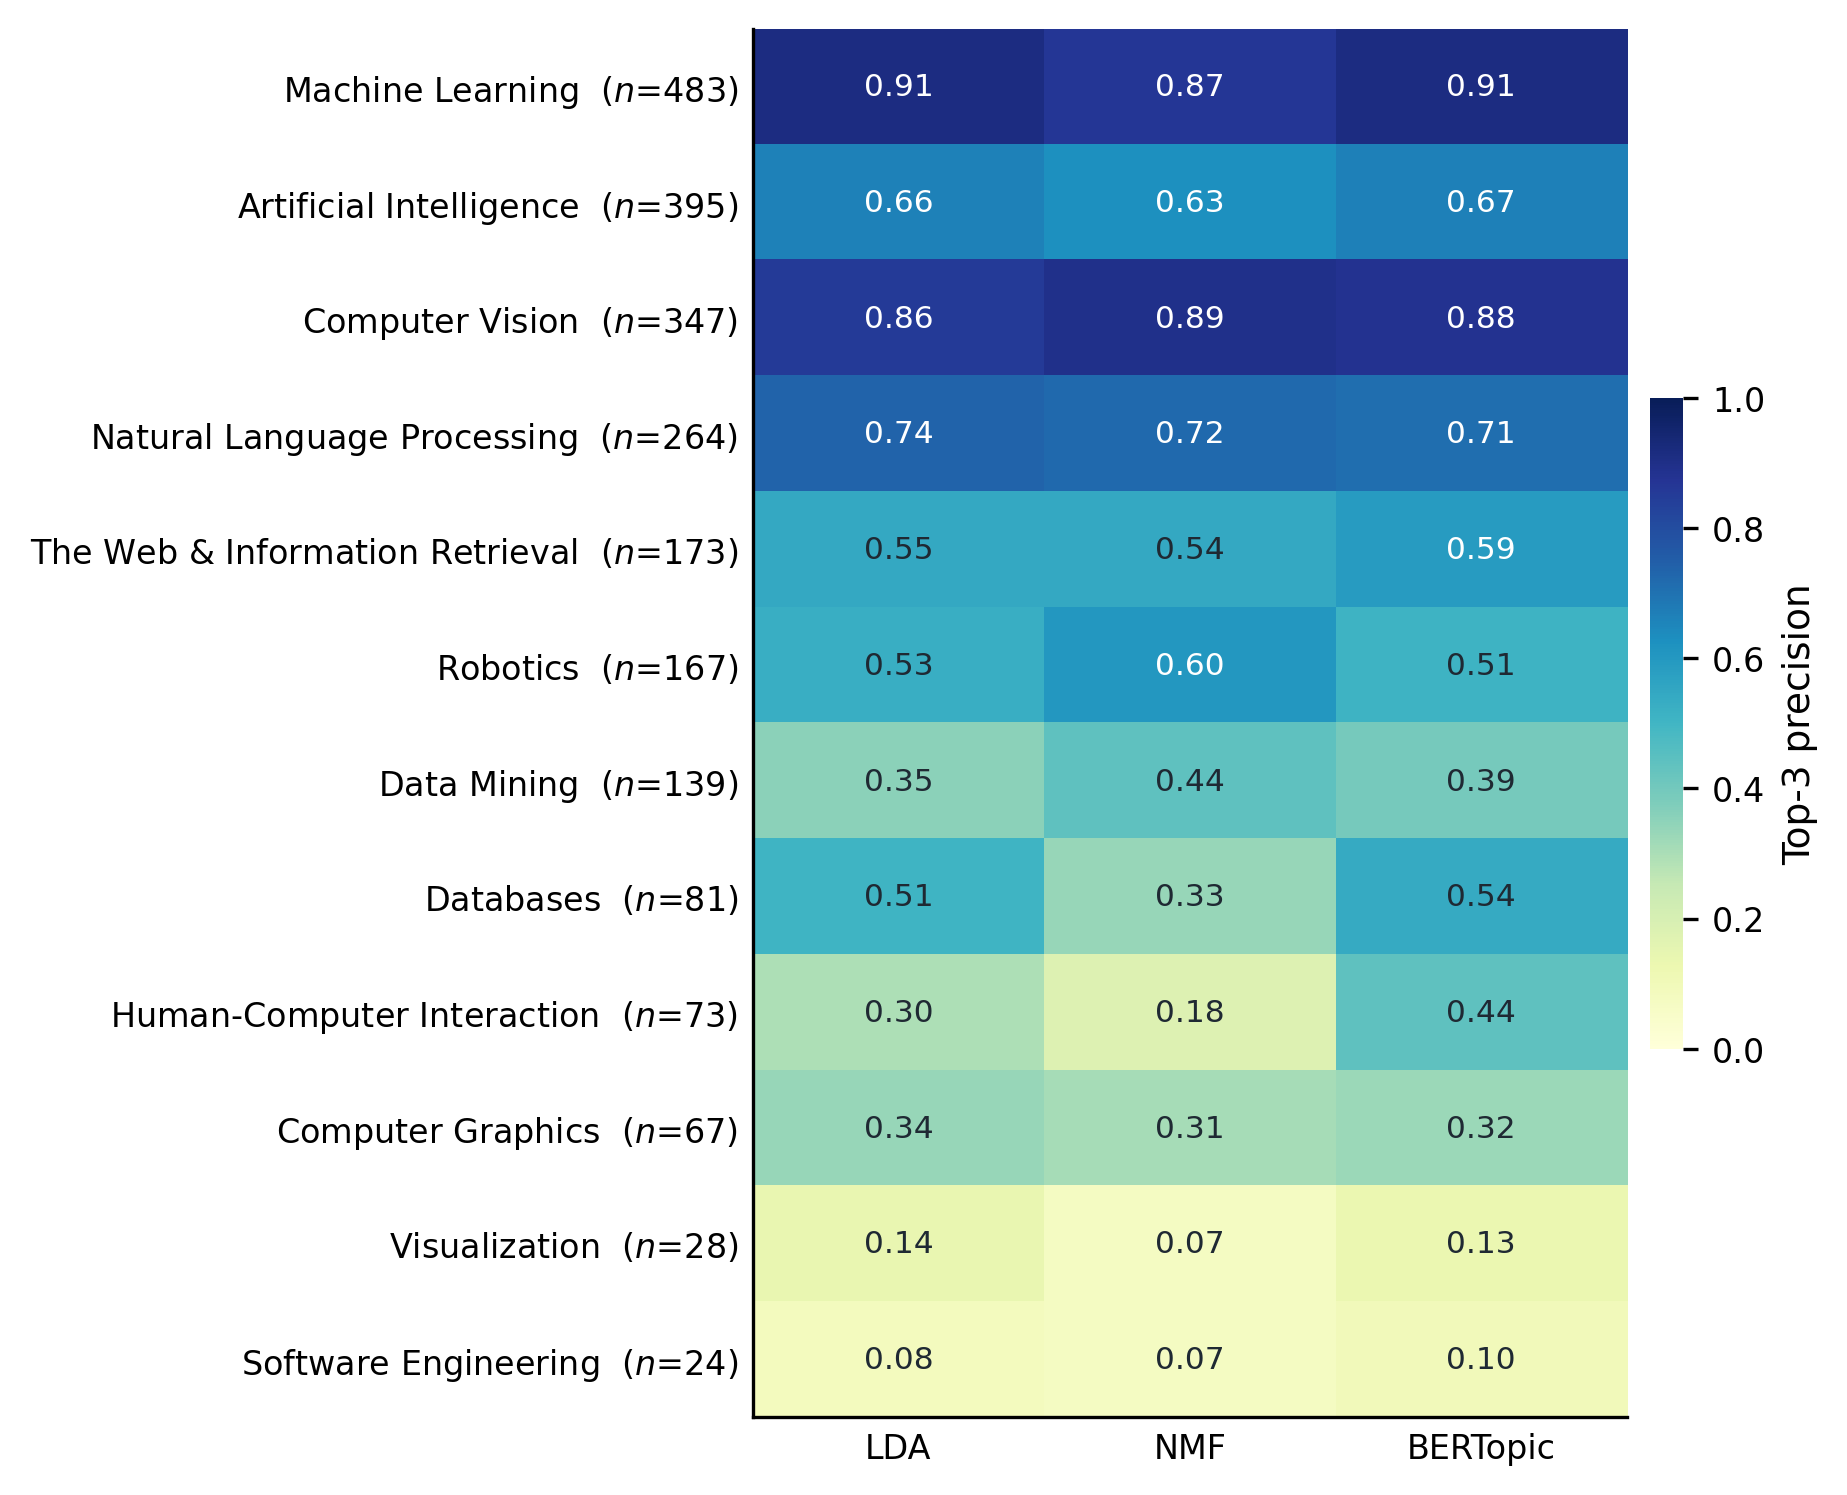
\includegraphics[width=0.94\columnwidth]{sections/figures/06_per_group_performance.png}
    \caption{Top-3 precision by research group.}
    \label{fig:pergroup}
\end{figure}

The smallest test groups recorded the lowest Top-3 precision: Visualization ($n=28$) scored 0.07--0.14 and Software Engineering ($n=24$) scored 0.07--0.10, while Computer Graphics stayed below 0.34 despite 67 relevant researchers; Databases, by contrast, reached 0.54 with BERTopic from 81 researchers, so group size alone did not explain the differences. Because Top-3 precision is a proportion from a small sample, its variability is largest where the group is smallest: a binomial standard error of $\sqrt{p(1-p)/n} \approx 0.05\text{--}0.06$ around a precision near 0.10 for Visualization and Software Engineering implies a 95\% confidence interval spanning most of the observed range, so their model orderings should be read as indicative rather than conclusive.


\section{Conclusion}
\label{sec:conclusion}
This study answers the two research questions posed in Section~\ref{sec:intro}, showing that publication-based topic representations can support researcher-to-research-group recommendation. BERTopic produced the numerically best ranking performance on every metric, though its margin over LDA was statistically significant on only 3 of 13 tested metrics (Section~\ref{sec:results}), while NMF was most efficient. The main contribution is a BERTopic-based framework representing publications, researchers, and research groups in a shared topic space; its novelty lies in the controlled comparison of LDA, NMF, and BERTopic rather than in a new algorithm, clarifying how topic representation affects ranking quality and showing that a numerical ranking alone does not establish which differences are statistically dependable.

Topic coherence is not a reliable substitute for downstream evaluation: NMF generated the most coherent topics but the weakest recommendations, while BERTopic's better ranking quality came at a much higher cost and may partly reflect its externally pretrained SPECTER embeddings rather than an intrinsic property of contextual topic modeling. Model selection should reflect intended use: BERTopic when quality has priority and offline training is acceptable, LDA as a reasonable default at a fraction of the cost when that fragile margin does not justify the expense, and NMF when frequent retraining or limited resources dominate, at the cost of recommendation quality.

The evaluation is limited to CSRankings data from 12 computer science research groups, one researcher-level split, and profiles derived only from titles and abstracts; it also does not separate BERTopic's contextual architecture from SPECTER's external pretraining, so results should be read as topic-modeling pipelines as commonly deployed rather than an ablation of the contextual mechanism. Uneven group sizes and publication counts may further affect profile quality, particularly for the smallest groups, limiting generalization beyond this dataset. The significance tests in Section~\ref{sec:results} quantify uncertainty within this split; future work should evaluate repeated splits, extend to additional institutions or disciplines, examine performance by profile size, test citation, collaboration, and temporal information and alternative aggregation, and ablate BERTopic's components to determine whether its advantage over LDA persists once the pretraining confound is controlled.


\section*{Acknowledgement}
The authors acknowledge the use of OpenAI Codex (GPT-5.6) as an AI coding assistant for code completion and debugging during the implementation of the experiments, as well as Google NotebookLM to support literature review and reference analysis during the preparation of this manuscript. All AI-assisted content was reviewed, verified, and revised by the authors, who assume full responsibility for the content of this paper.

\bibliographystyle{ieeetr}
\bibliography{myrefs}

\end{document}
